
% \vspace{-0.1in}
\section{Analysis}
% \hamed{for arxiving you don't have space limitation, so get rid of wrap figures. They are just annoying to deal with :-)}

\subsection{Different RL methods: PPO vs. GRPO}\label{sec:ppo-grpo}

We evaluate \Ours using both PPO and GRPO as the base RL method, conducting experiments on Qwen2.5-3B/7B models. The training dynamics comparison is presented in Figure \ref{fig:joint-study}(a) and the evaluation results are presented in Table \ref{tab:ppo-grpo}, revealing the following insights:
\textbf{(1) GRPO converges faster than PPO across all cases.} This is because PPO relies on a critic model, which requires several warm-up steps before effective training begins.
\textbf{(2) PPO demonstrates greater training stability.} As shown in Figure \ref{fig:joint-study}(a), GRPO leads to reward collapse after training for many steps, whereas PPO remains stable.
\textbf{(3) The final training rewards of PPO and GRPO are comparable.} Despite differences in convergence speed and stability, both methods achieve similar final train reward and performance, indicating that both are viable for optimizing \Ours.
% \textbf{(4) GRPO and PPO achieve comparable performance.} Across both Qwen2.5-3B and Qwen2.5-7B, PPO and GRPO perform similarly. 
PPO exhibits greater training stability, making it a preferable choice in this setting. 
More results are in Appendix \ref{sec:appendix:ppo-grpo}.


\begin{table}[t]
    \centering
    \scriptsize
    \setlength{\tabcolsep}{4pt}
    \renewcommand{\arraystretch}{1.2}
    \caption{The performance results of \Ours with PPO and GRPO on seven datasets.}\label{tab:ppo-grpo}
    \begin{tabular}{lcccccccc}
        \toprule
        \textbf{Method} & \textbf{NQ} & \textbf{TriviaQA} & \textbf{PopQA} & \textbf{HotpotQA} & \textbf{2wiki} & \textbf{Musique} & \textbf{Bamboogle} & \textbf{Avg.} \\
        
        \midrule
        \multicolumn{8}{l}{\textbf{Qwen2.5-7b-Base/Instruct}} \\
        \Ours-base (GRPO) & 0.395 & 0.560 & 0.388 & 0.326 & 0.297 & 0.125 & 0.360 & 0.350 \\
        \Ours-instruct (GRPO) & 0.429 & 0.623 & 0.427 & 0.386 & 0.346 & 0.162 & 0.400 & 0.396 \\
        \hdashline
        \Ours-base (PPO) & \textbf{0.480} & \textbf{0.638} & \textbf{0.457} & \textbf{0.433} & 0.382 &\textbf{ 0.196} & \textbf{0.432} & \textbf{0.431}  \\
        \Ours-instruct (PPO) &  0.393 & 0.610 & 0.397 & 0.370 & \textbf{0.414} & 0.146 & 0.368 & 0.385 \\

        \midrule
        \multicolumn{8}{l}{\textbf{Qwen2.5-3b-Base/Instruct}} \\
        \Ours-base (GRPO) & \textbf{0.421} & 0.583 & 0.413 & 0.297 & 0.274 & 0.066 & 0.128 & 0.312 \\
        \Ours-instruct (GRPO) & 0.397 & 0.565 & 0.391 & \textbf{0.331} & 0.310 & \textbf{0.124} & 0.232 & \textbf{0.336}  \\
        \hdashline
        \Ours-base (PPO) & 0.406 & \textbf{0.587} & \textbf{0.435} & 0.284 & 0.273 & 0.049 & 0.088 & 0.303  \\
        \Ours-instruct (PPO) & 0.341 & 0.545 & 0.378 & 0.324 & \textbf{0.319} & 0.103 & \textbf{0.264} & 0.325   \\
        \bottomrule
    \end{tabular}
\end{table}


\subsection{Base vs. Instruct LLMs}

We analyze the training dynamics of \Ours across both base LLMs and instruction-tuned LLMs. Experiments are conducted on two model variants: Qwen2.5-3B, and Qwen2.5-7B.
As shown in Figure \ref{fig:joint-study}(b), we observe that instruction-tuned models converge faster and start from a higher initial performance compared to base models. 
However, the final training reward of both model types remains highly similar after training. 
This finding suggests that while general post-training accelerates learning in reasoning-plus-search scenarios, RL can effectively bridge the gap over time, enabling base models to achieve comparable performance. More results can be found in Appendix \ref{sec:appendix:base-instruct}.



\begin{figure}[t]
    \centering
    \subfigure[PPO vs. GRPO]{%
        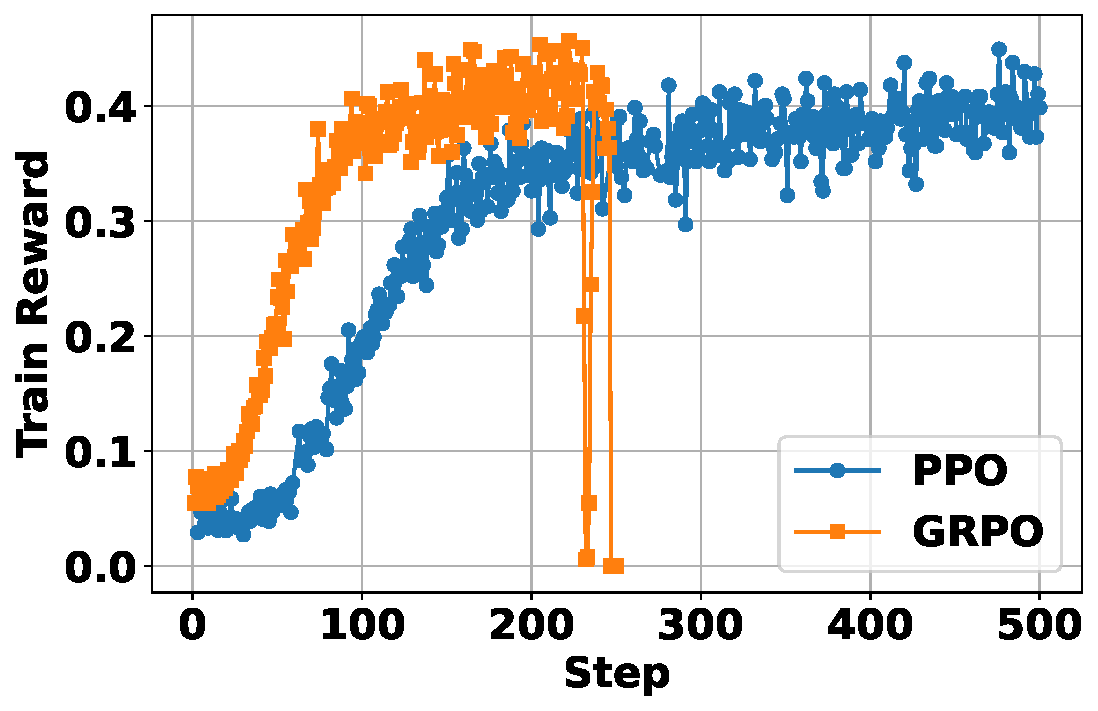
\includegraphics[width=0.225\textwidth]{figures/Search-R1_qwen-3b-base-ppo-grpo-new.pdf}
    }
    \subfigure[Base vs. Instruct]{%
        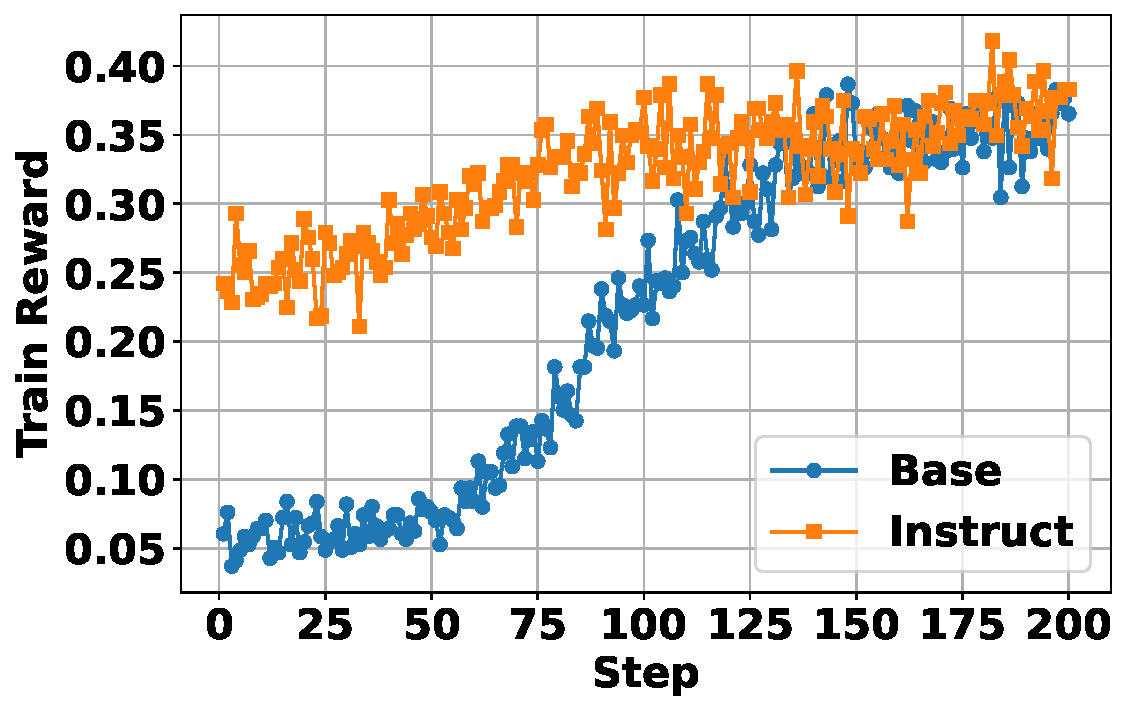
\includegraphics[width=0.225\textwidth]{figures/Search-R1_qwen-3b.pdf}
    }
    \subfigure[Response length]{%
        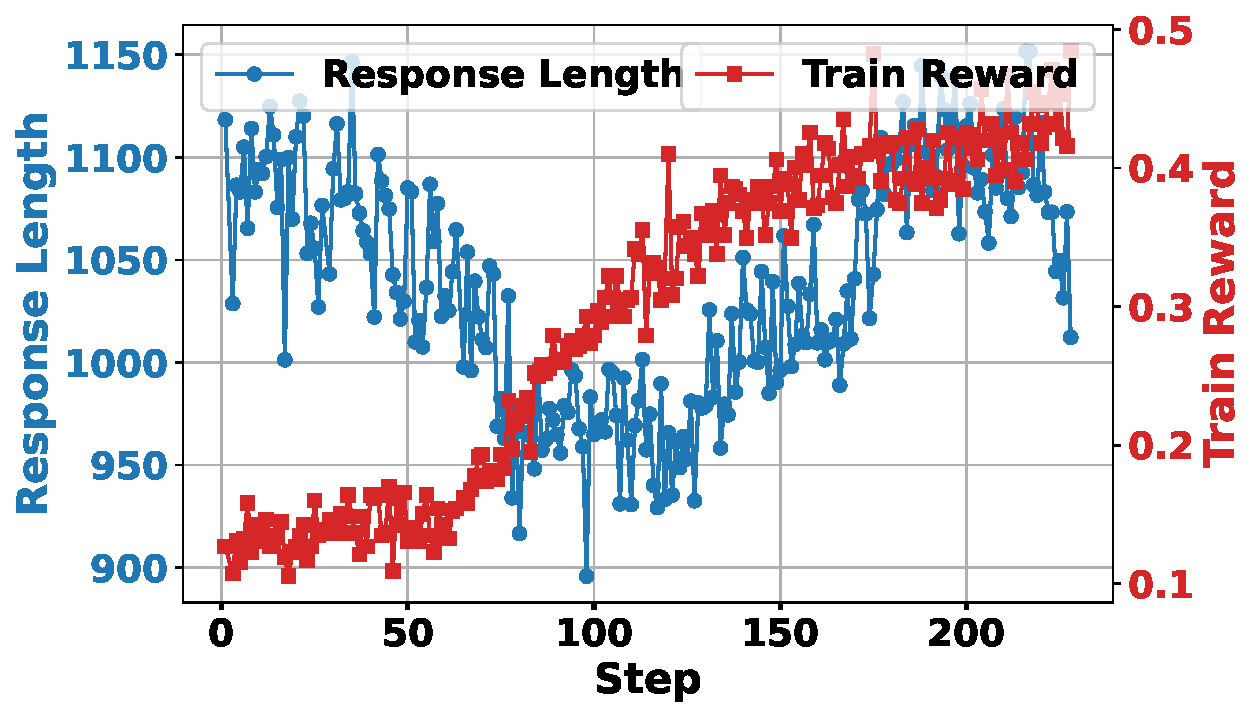
\includegraphics[width=0.255\textwidth]{figures/Search-R1_qwen-7b-response.pdf}
    }
    \subfigure[\# Valid search]{%
        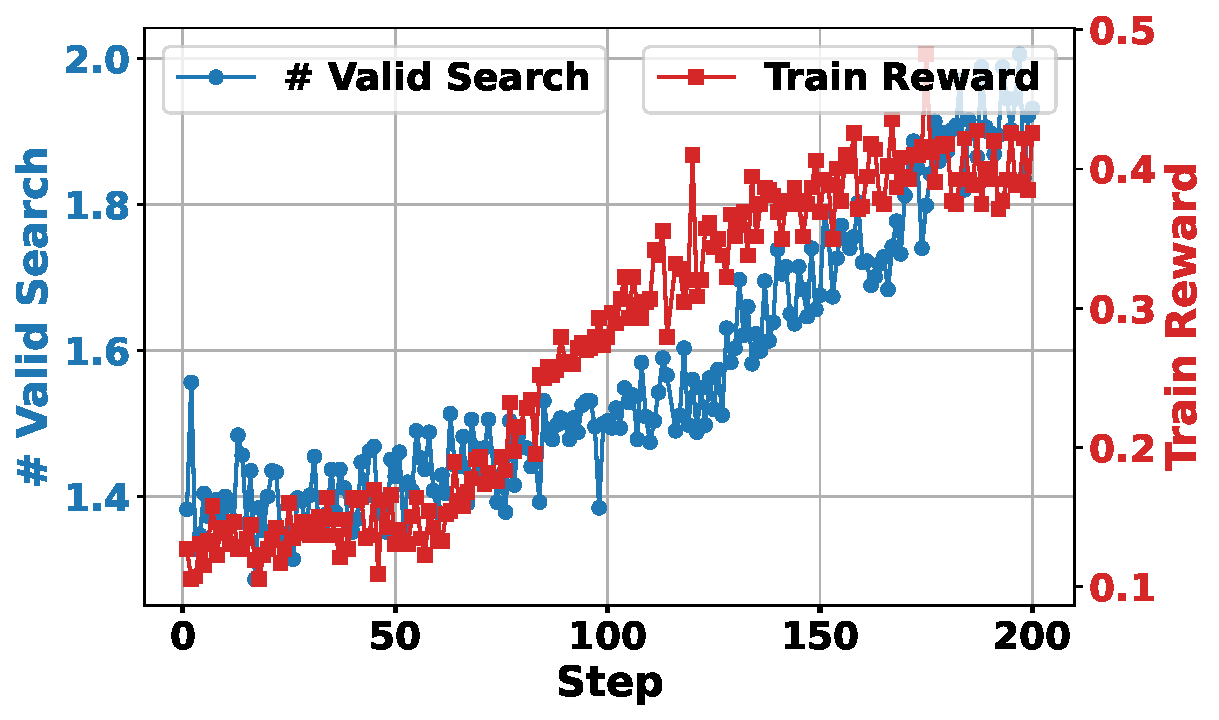
\includegraphics[width=0.25\textwidth]{figures/Search-R1_qwen-7b-valid-search.pdf}
    }
    % \subfigure[Loss mask]{%
    %     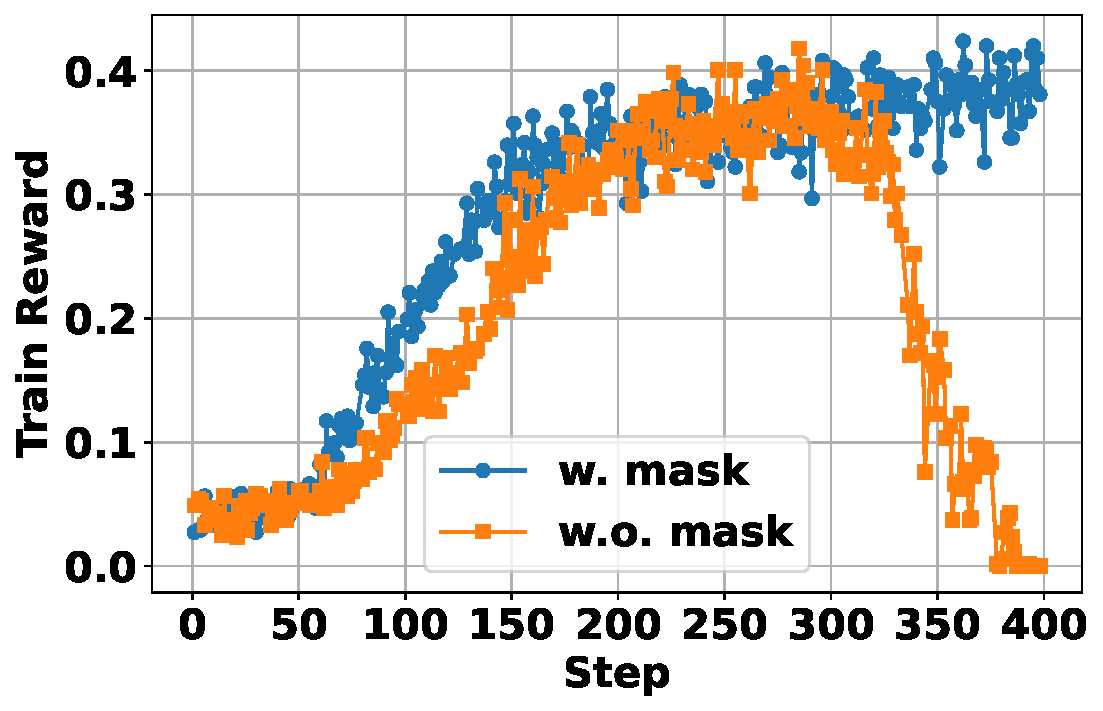
\includegraphics[width=0.225\textwidth]{figures/Search-R1_qwen3b-loss-mask.pdf}
    % }
    \vspace{-0.1in}
    \caption{
(a) PPO vs. GRPO: GRPO generally converges faster but may exhibit instability after trained
for a number of steps, whereas PPO provides more stable optimization but converges at a
slower rate.
(b) Base vs. Instruct LLM study: Instruction-tuned LLMs converge faster, but the final performance of both modles remains highly similar.
(c) Response length study: The response length exhibits a decrease-increase-stabilize trend throughout training, aligning with the overall performance trajectory of the LLM.
(d) \# Valid search study: As the training proceeds, the LLM learns to call search more.
% (d) Retrieved token loss masking study: Implementing retrieved token masking leads to greater LLM improvements, mitigating unintended optimization effects and ensuring more stable training dynamics.
}\label{fig:joint-study}
\vspace{-0.1in}
\end{figure}



\begin{table}[t]
    \centering
    \scriptsize
    \setlength{\tabcolsep}{3pt}
    \renewcommand{\arraystretch}{1.2}
    \caption{The performance of \Ours with and without retrieved token loss masking. The LLM trained with retrieved token loss masking achieves consistently better performance. (LLM: Qwen2.5-7b-base; RL: PPO)}\label{tab:loss-mask}
    \begin{tabular}{lcccccccc}
        \toprule
        \textbf{Method} & \textbf{NQ} & \textbf{TriviaQA} & \textbf{PopQA} & \textbf{HotpotQA} & \textbf{2wiki} & \textbf{Musique} & \textbf{Bamboogle} & \textbf{Avg.} \\
        \midrule
        % \multicolumn{8}{l}{\textbf{LLaMA3.2-3b-Base}} \\
        \Ours w. mask & \textbf{0.480} & \textbf{0.638} & \textbf{0.457}	& \textbf{0.433} & \textbf{0.382} & \textbf{0.196} & \textbf{0.432} & \textbf{0.431}  \\
        \Ours w.o. mask & 0.388 & 0.567 & 0.391	& 0.325 & 0.321 & 0.108 & 0.304 & 0.343 \\
        \bottomrule
    \end{tabular}
    \vspace{-0.1in}
\end{table}


\subsection{Response Length and Valid Search Study}

We conduct an experiment using \Ours with the Qwen2.5-7b-base model to analyze the dynamics of response length and number of valid search engine calls over the course of training. 
The response length result is presented in Figure \ref{fig:joint-study}(c), revealing the following key trends:
\textbf{(1) Early Stage (First 100 Steps)}: The response length sharply decreases, while the training reward exhibits a slight increase. During this phase, the base model learns to eliminate excessive filler words and begins adapting to the task requirements.
\textbf{(2) Later Stage (After 100 Steps)}: Both response length and training reward increase significantly. At this point, the LLM learns to call the search engine frequently, resulting in longer responses due to retrieved passages. The training reward improves substantially, as the model becomes more effective at leveraging search results.
The valid search result is presented in Figure \ref{fig:joint-study}(d), showing that the LLMs learn to call the search engine more times as the training proceeds.

\subsection{Study of Retrieved Tokens Loss Masking}

In Section \ref{sec:kl-mask}, we introduced loss masking for retrieved tokens to prevent unintended optimization behaviors. 
Here, we conduct experiments on the Qwen2.5-7b-base model, comparing training dynamics with and without retrieved token loss masking. 
As shown in Figure \ref{fig:apx:loss-mask}, applying retrieved token masking results in greater LLM improvements, mitigating unintended optimization effects and ensuring more stable training.
The performance comparison is provided in Table \ref{tab:loss-mask}, demonstrating that \Ours trained with retrieved token loss masking consistently outperforms the variant without masking.

More experimental results on retrieved token loss mask, base vs. instruct LLMs, comparison between PPO/GRPO, the number of retrieved passages in \Ours training, group size study in \Ours (GRPO), case studies can be found in Appendix \ref{apx:sec:retrieval-token}, \ref{sec:appendix:base-instruct}, \ref{sec:apx:topk}, \ref{apx:sec:grpo-size}, \ref{apx:sec:case1} and \ref{sec:apx:case-all}.
